\documentclass[aspectratio=169]{beamer}

% ── Clean theme base ─────────────────────────────────────
\usetheme{default}
\usecolortheme{default}

% ── Colors ───────────────────────────────────────────────
\definecolor{lightbg}{HTML}{ffffff}
\definecolor{examplebg}{HTML}{f5f5fa}
\definecolor{darktext}{HTML}{222222}
\definecolor{dimtext}{HTML}{777777}
\definecolor{accent}{HTML}{b8860b}
\definecolor{stage}{HTML}{2471a3}
\definecolor{warmred}{HTML}{c0392b}

% ── Light background + dark text ─────────────────────────
\setbeamercolor{background canvas}{bg=lightbg}
\setbeamercolor{normal text}{fg=darktext, bg=lightbg}
\setbeamercolor{frametitle}{fg=darktext, bg=lightbg}
\setbeamercolor{title}{fg=darktext}
\setbeamercolor{subtitle}{fg=dimtext}
\setbeamercolor{author}{fg=dimtext}
\setbeamercolor{date}{fg=dimtext}
\setbeamercolor{item}{fg=accent}
\setbeamercolor{subitem}{fg=dimtext}
\setbeamercolor{itemize item}{fg=accent}
\setbeamercolor{itemize subitem}{fg=dimtext}
\setbeamercolor{enumerate item}{fg=accent}
\setbeamercolor{block title}{fg=darktext, bg=lightbg}
\setbeamercolor{block body}{fg=darktext, bg=lightbg}
\setbeamercolor{structure}{fg=darktext}
\setbeamercolor{footline}{fg=dimtext}

% ── Fonts ────────────────────────────────────────────────
\setbeamerfont{frametitle}{size=\large, series=\bfseries}

% ── Remove chrome ────────────────────────────────────────
\setbeamertemplate{navigation symbols}{}
\setbeamertemplate{footline}{%
  \hfill{\color{dimtext}\tiny\insertframenumber}\hspace{14pt}\vspace{8pt}%
}
\setbeamertemplate{frametitle}{%
  \vspace{8pt}\insertframetitle%
}

\usepackage[utf8]{inputenc}
\usepackage{graphicx}

% ════════════════════════════════════════════════════════════
\begin{document}
\usebeamercolor[fg]{normal text}

% ── SLIDE 1: Title ───────────────────────────────────────
{
\setbeamertemplate{footline}{}
\begin{frame}
\vfill
\begin{center}
{\fontsize{36}{44}\selectfont\bfseries Where is this going?\par}
\vspace{20pt}
{\color{dimtext}\large The path from here to ColoredCow}
\vspace{30pt}


\includegraphics[width=0.18\textwidth]{coloredcow-logo.png}
\end{center}
\vfill
\end{frame}
}

% ── SLIDE 2: What we don't hire for ─────────────────────
\begin{frame}{}
\vfill
\begin{center}
\begin{minipage}{0.80\textwidth}
{\fontsize{22}{28}\selectfont We don't hire people who can code.\par}
\vspace{20pt}
{\fontsize{22}{28}\selectfont\color{warmred} AI can code.\par}
\vspace{20pt}
{\fontsize{22}{28}\selectfont We hire people who can \textbf{\color{accent}think},\par}
\vspace{4pt}
{\fontsize{22}{28}\selectfont take \textbf{\color{accent}ownership},\par}
\vspace{4pt}
{\fontsize{22}{28}\selectfont and \textbf{\color{accent}figure things out}.\par}
\end{minipage}
\end{center}
\vfill
\end{frame}

% ── SLIDE 4: Stage 1 ────────────────────────────────────
\begin{frame}{}
\vfill
\begin{center}
{\color{stage}\fontsize{18}{22}\selectfont STAGE 1\par}
\vspace{10pt}
{\fontsize{28}{34}\selectfont\bfseries Can you see a real problem?\par}
\vspace{30pt}
{\color{accent}\large $\rightarrow$ You are here right now.\par}
\vspace{30pt}
\begin{minipage}{0.80\textwidth}
{\color{darktext}Some of you wrote ``students face problems in college.''\par}
\vspace{8pt}
{\color{darktext}Some of you wrote about a specific person,\\a specific frustration, a specific moment.\par}
\vspace{16pt}
{\color{dimtext}The first one is a Google search.\par}
\vspace{4pt}
{\color{accent}\bfseries The second one is thinking.\par}
\end{minipage}
\end{center}
\vfill
\end{frame}

% ── SLIDE 4: Stage 1 Example ────────────────────────────
{
\setbeamercolor{background canvas}{bg=examplebg}
\begin{frame}{}
\vfill
\begin{center}
{\color{stage}\normalsize STAGE 1 --- Example\par}
\vspace{16pt}
\begin{minipage}{0.82\textwidth}
{\color{darktext}I asked one of you:\par}
\vspace{8pt}
{\large\color{accent}``Who exactly has this problem?''\par}
\vspace{16pt}
{\color{dimtext}First answer: ``Students.''\par}
\vspace{12pt}
{\color{darktext}I asked again.\par}
\vspace{12pt}
{\color{darktext}Second answer: ``A student with rank 15,000 who has to choose between a low-branch IIT and a top-branch NIT, and his father only trusts the IIT tag.''\par}
\vspace{20pt}
{\color{accent}\bfseries That second answer is Stage 1 done right.\par}
\end{minipage}
\end{center}
\vfill
\end{frame}
}

% ── SLIDE 6: We don't expect perfection ─────────────────
\begin{frame}{}
\vfill
\begin{center}
{\fontsize{26}{32}\selectfont\bfseries We don't expect perfection.\par}
\vspace{30pt}
\begin{minipage}{0.80\textwidth}
{\color{darktext}We are not looking for the perfect problem statement.\par}
\vspace{14pt}
{\color{darktext}We are looking for the right direction. Are you thinking clearly? Are you asking real questions? Are you going deeper when pushed?\par}
\vspace{14pt}
{\color{accent}\bfseries That is enough. Keep going.\par}
\end{minipage}
\end{center}
\vfill
\end{frame}

% ── SLIDE 7: Stage 2 ────────────────────────────────────
\begin{frame}{}
\vfill
\begin{center}
{\color{stage}\fontsize{18}{22}\selectfont STAGE 2\par}
\vspace{8pt}
{\fontsize{28}{34}\selectfont\bfseries Can you keep going without us?\par}
\vspace{20pt}
\begin{minipage}{0.80\textwidth}
{\color{darktext}We are here this week. But we will leave.\par}
\vspace{10pt}
{\color{darktext}After we leave, do you keep working on your problem?\par}
\vspace{4pt}
{\color{darktext}Do you come back with progress that\\no one asked you for?\par}
\vspace{14pt}
{\color{accent}\bfseries This is ownership.\par}
\vspace{4pt}
{\color{dimtext}Not waiting for instructions. Moving on your own.\par}
\end{minipage}
\end{center}
\vfill
\end{frame}

% ── SLIDE 6: Stage 2 Example ────────────────────────────
{
\setbeamercolor{background canvas}{bg=examplebg}
\begin{frame}{}
\vfill
\begin{center}
{\color{stage}\normalsize STAGE 2 --- Example\par}
\vspace{16pt}
\begin{minipage}{0.82\textwidth}
{\color{darktext}One of you wrote the feedback problem.\\We asked you tough questions.\\You realized your problem was not clear enough.\par}
\vspace{14pt}
{\color{accent}Stage 2 is:\par}
\vspace{8pt}
{\color{darktext}Next week, without anyone telling you, you go talk to 5 classmates and ask them---\par}
\vspace{6pt}
{\large\color{accent}``When was the last time you wanted to give feedback about a teacher but didn't? Why?''\par}
\vspace{14pt}
{\color{darktext}You come back with real answers.\par}
\vspace{4pt}
{\color{dimtext}No one asked you to do this.\par}
\vspace{4pt}
{\color{accent}\bfseries You did it because the problem is yours now.\par}
\end{minipage}
\end{center}
\vfill
\end{frame}
}

% ── SLIDE 7: Stage 3 ────────────────────────────────────
\begin{frame}{}
\vfill
\begin{center}
{\color{stage}\fontsize{18}{22}\selectfont STAGE 3\par}
\vspace{10pt}
{\fontsize{26}{32}\selectfont\bfseries You start working with us.\par}
\vspace{30pt}
\begin{minipage}{0.80\textwidth}
{\color{darktext}If you show Stage 1 and Stage 2, we give you something real to work on.\par}
\vspace{14pt}
{\color{darktext}Things like our website, or tools we are building for our team. Real work, real users, real impact. But with room to learn and make mistakes.\par}
\vspace{14pt}
{\color{dimtext}This is not ``go write code.''\par}
\vspace{4pt}
{\color{accent}\bfseries This is: can you think about the problem, understand the user, and figure out what to do?\par}
\end{minipage}
\end{center}
\vfill
\end{frame}

% ── SLIDE 8: Stage 3 Example ────────────────────────────
{
\setbeamercolor{background canvas}{bg=examplebg}
\begin{frame}{}
\vspace{2pt}
\begin{center}
{\color{stage}\normalsize STAGE 3 --- Example\par}
\vspace{8pt}
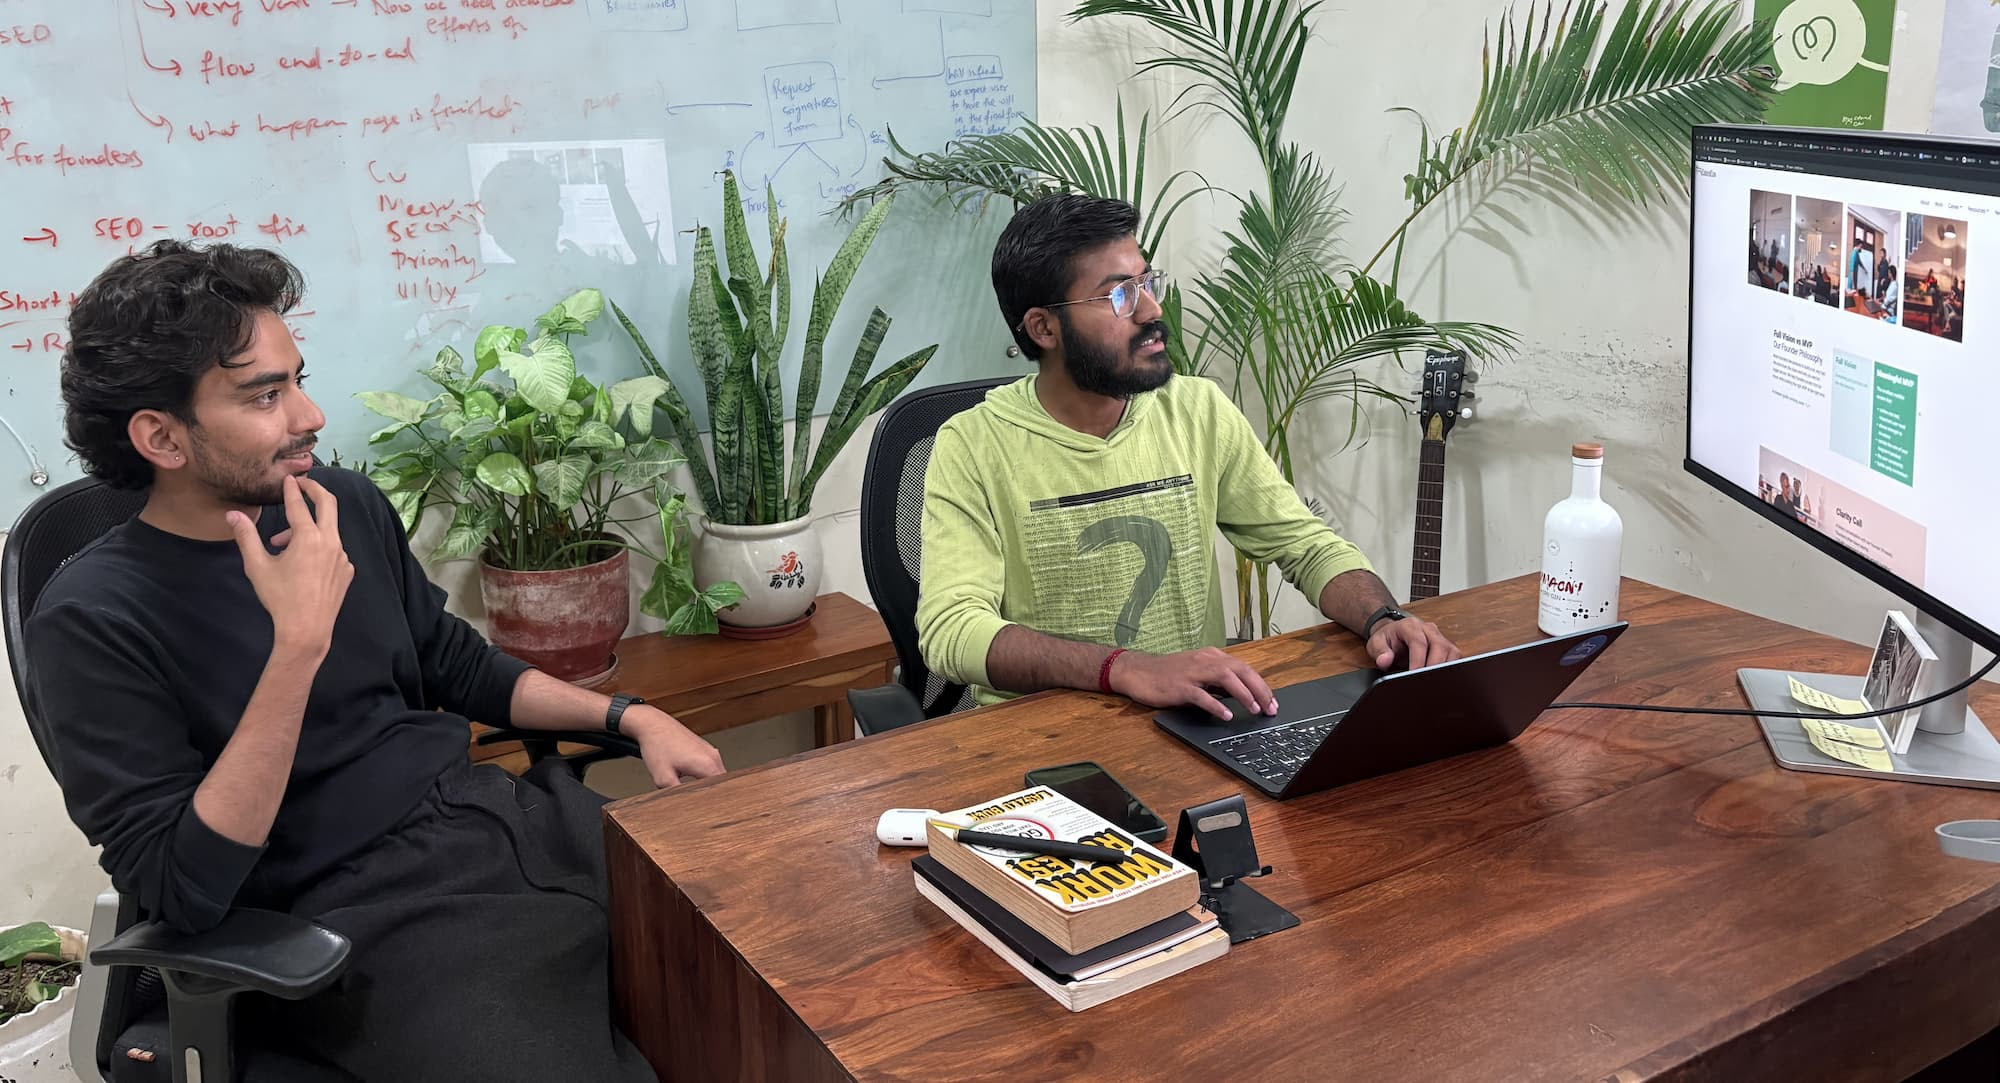
\includegraphics[width=0.65\textwidth]{soumyadip-hitesh-coloredcow.jpg}\\[14pt]
\begin{minipage}{0.65\textwidth}
\centering
{\small\color{darktext}\textbf{Soumyadip} from GKV, working with \textbf{Hitesh}, our designer, on the ColoredCow website.\par}
\vspace{4pt}
{\small\color{darktext}Not a practice project. \textbf{\color{accent}Our actual website.}\par}
\vspace{4pt}
{\small\color{dimtext}He got here by showing he could think and take ownership.\par}
\end{minipage}
\end{center}
\end{frame}
}

% ── SLIDE 9: Stage 4 ────────────────────────────────────
\begin{frame}{}
\vfill
\begin{center}
{\color{stage}\fontsize{18}{22}\selectfont STAGE 4\par}
\vspace{10pt}
{\fontsize{26}{32}\selectfont\bfseries You earn a seat on a real project.\par}
\vspace{30pt}
\begin{minipage}{0.80\textwidth}
{\color{darktext}When you show strong thinking in the playground, when you take ownership, when you push things forward without being told---\par}
\vspace{14pt}
{\color{darktext}You get a chance to work on an actual client project alongside our team.\par}
\vspace{14pt}
{\color{accent}\bfseries Real clients. Real stakes. Real impact.\par}
\end{minipage}
\end{center}
\vfill
\end{frame}

% ── SLIDE 13: What "ready" looks like ───────────────────
\begin{frame}{}
\vfill
\begin{center}
{\fontsize{26}{32}\selectfont\bfseries What ``ready'' looks like.\par}
\vspace{30pt}
\begin{minipage}{0.80\textwidth}
{\color{darktext}Ready does not mean you know everything about the project.\par}
\vspace{14pt}
{\color{darktext}Ready means: we are confident that you understand our problem. That you will approach each project differently. That you will not walk in and ask ``tell me what to do'' or ``assign me tasks I can complete.''\par}
\vspace{14pt}
{\color{darktext}Ready means: you see the problem, you think about it, and you figure out your move.\par}
\vspace{14pt}
{\color{dimtext}The code is not the output we want.\par}
\vspace{4pt}
{\color{accent}\bfseries The thinking is.\par}
\end{minipage}
\end{center}
\vfill
\end{frame}

% ── SLIDE 14: Stage 5 ───────────────────────────────────
\begin{frame}{}
\vfill
\begin{center}
{\color{stage}\fontsize{18}{22}\selectfont STAGE 5\par}
\vspace{8pt}
{\fontsize{24}{30}\selectfont\bfseries You become someone we can't\par}
\vspace{2pt}
{\fontsize{24}{30}\selectfont\bfseries imagine working without.\par}
\vspace{18pt}
\begin{minipage}{0.80\textwidth}
{\color{accent}\large This is when placement happens.\par}
\vspace{10pt}
{\color{darktext}Not because you passed a test.\par}
\vspace{6pt}
{\color{darktext}Because over weeks and months,\\through your thinking, your ownership, and your work,\\you became part of the team.\par}
\vspace{12pt}
{\color{dimtext}Placement at ColoredCow is not a gate.\par}
\vspace{4pt}
{\color{accent}\bfseries It is a relationship that builds over time.\par}
\end{minipage}
\end{center}
\vfill
\end{frame}

% ── SLIDE 11: Where you are ─────────────────────────────
\begin{frame}{}
\vfill
\begin{center}
{\fontsize{30}{36}\selectfont\bfseries You are in Stage 1.\par}
\vspace{30pt}
{\large\color{darktext}How seriously you take it\\decides whether Stage 2 happens.\par}
\vspace{30pt}
{\color{dimtext}The problem statement you wrote?\par}
\vspace{4pt}
{\color{dimtext}That is not an assignment.\par}
\vspace{12pt}
{\color{accent}\fontsize{22}{28}\selectfont\bfseries That is your Stage 1.\par}
\end{center}
\vfill
\end{frame}

\end{document}
